\documentclass[a4paper,11pt]{article}
% FONTS and SYMBOLS %%%%%%%%%%%%%%%%%%%%%%%%%%%%%%%
\usepackage[utf8]{inputenc}
\usepackage[francais]{babel}
%\usepackage[utf8]{inputenc}  
\usepackage[T1]{fontenc}
\usepackage{slantsc}
\usepackage{lmodern}
\usepackage{textcomp}
% USUAL GRAPHICAL TOOLS %%%%%%%%%%%%%%%%%%%%%%%%%%%
\usepackage{boxedminipage}
\usepackage{graphicx}
\usepackage[dvipsnames]{xcolor}
\usepackage{hyperref}

% PAGE LAYOUT %%%%%%%%%%%%%%%%%%%%%%%%%%%%%%%%%%%%%
%\textwidth 16cm
%\textheight 25.5cm
%\voffset -3cm
%\hoffset -2cm
%\parindent 0mm

\ttfamily
\newcommand{\lfont}{\fontseries{l}\selectfont}
\newcommand{\mfont}{\fontseries{m}\selectfont}
\newcommand{\bfont}{\fontseries{b}\selectfont}

% COLORS %%%%%%%%%%%%%%%%%%%%%%%%%%%%%%%%%%%%%%%%%%
\definecolor{file}{RGB}{215,230,255}
\definecolor{method}{RGB}{240,240,200}
\definecolor{variable}{RGB}{215,255,230}
% COLORS %%%%%%%%%%%%%%%%%%%%%%%%%%%%%%%%%%%%%%%%%%
\newcommand{\cod}[1]{{\ttfamily #1}}
\newcommand{\class}[2]{\par\vspace{1mm}\hspace{-5mm}\large\colorbox{file}{\textbullet\bfont\cod{#1}:} (\cod{#2})\par}
\newcommand{\method}[1]{\par\vspace{1mm}\hspace{-2mm}\colorbox{method}{\textopenbullet\bfont\cod{#1}:}}
\newcommand{\variable}[1]{\par\vspace{1mm}\hspace{-2mm}\colorbox{variable}{\textopenbullet\bfont\cod{#1}:}}



\usepackage{amsmath}
\usepackage{latexsym}
\usepackage{amsfonts}
\usepackage{amssymb}
\usepackage{graphicx}
\usepackage{txfonts}
\usepackage{wasysym}
\usepackage{adjustbox}
\usepackage{ragged2e}
\usepackage{tabularx}
\usepackage{hhline}
\usepackage{float}
\usepackage{multirow}
\usepackage{makecell}
\usepackage{fancyhdr}
\usepackage[utf8]{inputenc}
\usepackage[T1]{fontenc}
\usepackage[a4paper,bindingoffset=0.2in,headsep=0.5cm,left=1in,right=1in,bottom=3cm,top=2cm,headheight=2cm]{geometry}
\usepackage{hyperref}
\usepackage{listings}
\usepackage{color}

\definecolor{pblue}{rgb}{0.13,0.13,1}
\definecolor{pgreen}{rgb}{0,0.5,0}
\definecolor{pred}{rgb}{0.9,0,0}
\definecolor{pgrey}{rgb}{0.46,0.45,0.48}

\everymath{\displaystyle}
\pagestyle{fancy}
\fancyhf{}
\rfoot{Page \thepage}

\lstset{language=C,basicstyle=\footnotesize,keywordstyle=\color{red}\bfseries,  commentstyle=\color{blue}\textit,stringstyle=\color{green}\ttfamily, showspaces=false,showstringspaces=false}


\begin{document}
\sloppy 

\begin{center}
\Large Telecom Paris \\
\Large COMELEC Department \\
\vspace{20 pt}
\underline{\Huge TTool: Simulator of DIPLODOCUS}
\end{center}

\begin{table}[H]
\large
\centering
\begin{adjustbox}{width=\textwidth}
\begin{tabular}{ |p{1.6cm}|p{6.0cm}|p{4.4cm}|p{4.2cm}| }
\hhline{----}
 & \textbf{Document Manager} & \textbf{Contributors}  & \textbf{Checked by}  \\ 
\hhline{----}
\textbf{Name}   & Sophie COUDERT & Sophie COUDERT &
\multirow{2}{*}{Ludovic APVRILLE} \\
\hhline{--~~}
\textbf{Contact} & sophie.coudert@telecom-paris.fr & \multirow{2}{*}{} &  \\ 
\hhline{--~~}
\textbf{Date} & \today & Ludovic APVRILLE &  \\ 
\hline
\end{tabular}
\end{adjustbox}
\end{table}

\begin{figure}[!h]
\centering

\includegraphics[width=0.3\textwidth]{images/tp}
\end{figure}

\newpage
\tableofcontents

% \newpage
% \listoffigures

\newpage
\section{Preface}

\subsection{Table of Versions}

\begin{table}[H]
\large
\centering
\begin{adjustbox}{width=\textwidth}
\begin{tabular}{ |p{1.5cm}|p{2.5cm}|p{9.0cm}|p{3.0cm}| }
\hhline{----}
\textbf{Version} & \textbf{Date} & \textbf{Description  $  \&  $  Rationale of
Modifications} & \textbf{Sections Modified} \\
\hhline{----}
1.0 & 03/03/2022 & First draft &  \\ 
\hline
\end{tabular}
\end{adjustbox}
\end{table}

\subsection{Table of References and Applicable Documents}

\begin{table}[H]
\large
\centering
\begin{adjustbox}{width=\textwidth}
\begin{tabular}{ |p{2.66in}|p{2.66in}|p{0.95in}|p{0.43in}| }
\hhline{----}
\textbf{Reference} & \textbf{Title  $  \&  $  Edition} & \textbf{Author or
Editor} & \textbf{Year}
\\
\hhline{----}
 &  &  &  \\ 
\hline
\end{tabular}
\end{adjustbox}
\end{table}

\subsection{Acronyms and glossary}

\begin{table}[H]
\large
\centering
\begin{adjustbox}{width=\textwidth}
\begin{tabular}{ |p{1.24in}|p{5.45in}| }
\hhline{--}
\textbf{Term} & \textbf{Description} \\ 
\hhline{--}
 &  \\ 
\hline
\end{tabular}
\end{adjustbox}
\end{table}

\subsection{Executive Summary}

This document describes the structure and meaning of the code of the DIPLODOCUS simulator. General algorithms as well as individual methods of C++ classes are commented.

\newpage 

%$$$$$$$$$$$$$$$$$$$$$$$$$$$$$$$$$$$$$$$$$$$$$$$$$$$$$$$$$$$$$$$$$$$$$$$$$
%\begin{document}
%@@@@@@@@@@@@@@@@@@@@@@@@@@@@@@@@@@@@@@@@@@@@@@@@@@@@@@@@@@@@@@@@@@@@@
\section*{Base Directory \cod{src\_simulator}}
%===========================================
\class{Transaction}{}
%-----------------------
\variable{\_command} Transaction's command
%-----------------------
\variable{\_channel} Transaction's channel. Relevant for communication transactions.
%-----------------------
\variable{\_runnableTime} Time at which the transaction is allowed to start. May be in the future, for example after a static delay.
%-----------------------
\variable{\_startTime} transaction's actual start time. Progressively updated while trying to execute, until transaction is actually executed (in particular for bus transaction).
%-----------------------
\variable{\_virtualLength} number of execution units of the transaction, i.e. bytes for communication transaction and integer instructions for exec-similar commands. Also progressively updated.
%-----------------------
\variable{\_length} length with "real" time as unit (cycles??). Also progressively updated.
%-----------------------
\variable{\_idlePenalty} time (cycle) updated while simulating.
%-----------------------
\variable{\_taskSwitchingPenalty} time (cycle) updated while simulating.
%-----------------------
\variable{\_transactCoreNumber} core that executes transaction (when multicore CPU).
%-----------------------
\variable{\_transType} among \cod{NOCOMM\_TRANS}: transactions without communication, \cod{CHANNEL\_TRANS}: transaction on event channel, \cod{BUS\_TRANS\_NoLength}: data communication on bus where length is not up-to-date, \cod{BUS\_TRANS\_Length}: data communication on bus whith length up-to-date. Initialised in \cod{calcStartTimeLength} of CPUS and finalised (for length) in CPU's \cod{getNextTransaction} (when last bus master of channel is granted).
%-----------------------
\method{getStartTimeOperation()} takes penalties into account
%-----------------------
\method{getEndTime()} takes penalties into account

%@@@@@@@@@@@@@@@@@@@@@@@@@@@@@@@@@@@@@@@@@@@@@@@@@@@@@@@@@@@@@@@@@@@@@
\section*{Directory \cod{app}}

%£££££££££££££££££££££££££££££££££££££££££££££££££££££££££££££££££££££
\subsection*{Channels}
%===========================================
\class{TMLChannel}{}
Class for mapped channels.
%-----------------------
\variable{\_width} Channel size (in bytes)

%-----------------------
\variable{\_readTask} tasks which performs read operation on the channel

%-----------------------
\variable{\_writeTask} tasks which performs write operation on the channel

%-----------------------
\variable{\_writeTrans} transaction which attempts to write in the channel

%-----------------------
\variable{\_readTrans} transaction which attempts to read the channel

%-----------------------
\variable{\_masters} buses on which the channel is mapped. doubble list: from first write master to last one, then from last read master to first one. Thus the last write master is repeated (equal to the last read master because on the same memory), which is used to detect the memory position.

%-----------------------
\variable{\_slaves} slaves on which the channel is mapped. Respects order of masters.

%-----------------------
\variable{\_writeTransCurrHop} current Hop (master/slave) of write Transaction
	
%-----------------------
\variable{\_readTransCurrHop} current Hop (master/slave) of read Transaction
	
%-----------------------
\method{testWrite(iTrans)} Prepares a write operation (depends on channel type)

%-----------------------
\method{testRead(iTrans)} Prepares a read operation (depends on channel type)

%-----------------------
\method{write()} Performs the write operation (depends on channel type)

%-----------------------
\method{read()} returns bool. Performs the read operation (depends on channel type)

%-----------------------
\method{getNextMaster(iTrans)} Returns the next communication master on which the given transaction is conveyed. Supposes that \cod{iTrans} is \cod{\_writeTrans} or \cod{\_readTrans}. First increments \cod{\_writeTransCurrHop} or decrements \cod{\_readTransCurrHop}. Returns the newly pointed master.
%-----------------------
\method{isLastMaster(iTrans)} Returns true if the current communication master (\cod{xxxCurrHop}) on which the given transaction is conveyed is the last one. Does not modify \cod{xxxCurrHop}.

%-----------------------
\method{getFirstMaster(iTrans)} Returns the first communication master on which the given transaction is conveyed. Supposes that \cod{iTrans} is \cod{\_writeTrans} or \cod{\_readTrans}. Set (read or write) current hop to this master.

%-----------------------
\method{getNextSlave(iTrans)} Returns the next slave component to which the given transaction is sent. Supposes that \cod{iTrans} is \cod{\_writeTrans} or \cod{\_readTrans}. Returns slave without modifying hops.

%===========================================
\class{TMLStateChannel}{TMLChannel}
Class for mapped channels with content (FIFOs). There are also data to handle losses of samples in the channel, which are abstracted here.

%-----------------------
\variable{\_content} Content of the channel

%-----------------------
\variable{\_nbToWrite} Number of samples the write transaction attempts to write

%-----------------------
\variable{\_nbToRead} Number of samples the read transaction attempts to read
	
%-----------------------
\variable{\_overflow} Buffer overflow flag
	
%-----------------------
\variable{\_underflow} Buffer underflow flag
	

%===========================================
\class{TMLbrbwChannel}{TMLStateChannel}
Blocking read-blocking write. Handling of losses is abstracted.
%-----------------------
\method{setTransactionLength()} Determines the virtual length of read and write transactions based on the state of the channel. Updates \cod{\_readTrans} and\cod{\_writeTrans}'s virtual lengthes, \cod{\_overflow} and \cod{\_underflow}. Chooses the maximal length respecting demanded length and content/place, but split it at the size that allows the symetric operation to fully execute if relevant and possible (when \cod{\_nbToRead}$>${\_content} ($\Rightarrow$ \cod{\_underflow}={\tt true}), or \cod{\_nbToWrite}$>$\cod{length $-$\_content} ($\Rightarrow$\cod{\_overflow}={\tt true})).

%-----------------------
\method{testWrite(iTrans)} updates \cod{\_nbToWrite} and \cod{\_writeTrans}. Then calls \cod{setTransac\-tion\-Length}.

%-----------------------
\method{testRead(iTrans)} updates \cod{\_nbToRead} and \cod{\_readTrans}. Then calls \cod{setTransaction\-Length}.

%-----------------------
\method{write()} called after \cod{testWrite}, thus number of samples is known and allowed (\cod{\_wri\-te\-Trans}'s virtual length). Updates \cod{\_content} and unblock \cod{\_readTrans} (set its runnable time). Reset (to 0) \cod{\_nbToRead} and \cod{\_nbToWrite}, then calls \cod{setTransactionLength}. Losses are handled here.
%-----------------------
\method{read()} called after \cod{testRead}, thus number of samples is known and allowed (\cod{\_read\-Trans}'s virtual length). Returns {\tt false} if \cod{\_content} $<$ \cod{\_readTrans}'s virtual length. Otherwise, returns {\tt true}, updates  \cod{\_content} and unblock \cod{\_writeTrans} (set its runnable time). Reset (to 0) \cod{\_nbToRead} and \cod{\_nbToWrite}, then calls \cod{setTransactionLength}.
%-----------------------
\method{getBlockedReadTask(),getBlockedWriteTask()}
%===========================================
\class{TMLbrnbwChannel}{TMLStateChannel}
Blocking read-non blocking write. Handling of losses is abstracted.
%-----------------------
\method{setTransactionLength()} Determines the virtual length of read and write transactions based on the state of the channel. Updates \cod{\_readTrans} and\cod{\_writeTrans}'s virtual lengthes and \cod{\_underflow}. Chooses the maximal length respecting demanded length and content/place, but split it at the size that allows the symetric operation to fully execute if relevant and possible (when \cod{\_nbToRead}$>${\_content} ($\Rightarrow$ \cod{\_underflow}={\tt true})).

%-----------------------
\method{testWrite(iTrans), testRead(iTrans), write()} similar to \cod{TMLbrbwChannel}.

%-----------------------
\method{read()} called after \cod{testRead}, thus number of samples is known and allowed (\cod{\_read\-Trans}'s virtual length). returns {\tt false} if \cod{\_content} $<$ \cod{\_readTrans}'s virtual length. Returns {\tt false} if \cod{\_content} $<$ \cod{\_readTrans}'s virtual length. Otherwise, returns {\tt true}, updates  \cod{\_content} and reset \cod{\_nbToRead} and \cod{\_nbToWrite}.
%-----------------------
\method{getBlockedReadTask(),getBlockedWriteTask()}

%===========================================
\class{TMLnbrnbwChannel}{TMLChannel}
Non blocking read-non blocking write

%-----------------------
\method{testWrite(iTrans), testRead(iTrans)} respectively update \cod{\_wri\-teTrans} and \cod{\_readTrans}.

%-----------------------
\method{write(iTrans), read(iTrans)} respectively reset (to 0) \cod{\_wri\-te\-Trans} and \cod{\_readTrans}.

%===========================================
\class{TMLEventChannel}{TMLStateChannel}
%-----------------------
\method{cancelReadTransaction()} Cancels a pending read operation 
%-----------------------
\method{{\rm virtual} write(iTrans), write()} \cod{write} calls \cod{write(this)} and resets \cod{\_writeTrans}.
%-----------------------
\method{getRequestChannel()} test channel's type. returns bool, default 0.
%-----------------------
\method{getBlockedReadTask(),getBlockedWriteTask()}

%===========================================
\class{TMLEventSizedChannel}{TMLEventChannel}
%-----------------------
\variable{\_paramQueue} Queue for parameters
%-----------------------
\variable{\_tmpParam} Temporary buffer for the parameters of the registered write transaction.

%===========================================
\class{TMLEventFChannel}{TMLEventSizedChannel}
Blocking read non blocking write. Samples which do not fit in the channel are dropped

%-----------------------
\variable{\_length}Length of the channel
%-----------------------
\method{testWrite(iTrans)}
Updates \cod{\_writeTrans}, \cod{\_tmpParam} (from \cod{iTrans}'s command), \cod{\_writeTrans}'s virtual length (fixed constant WAIT\_SEND\_VLEN) and \cod{\_overflow} (set to {\tt true} when \cod{\_content} is \cod{\_length}. );

%-----------------------
\method{testRead(iTrans)}
Updates \cod{\_readTrans},  \cod{\_readTrans}'s virtual length (fixed constant WAIT\_SEND\_VLEN, if channel not empty), \cod{\_readTrans}'s channel and \cod{\_underflow} ({\tt true} if channel is empty);

%-----------------------
\method{write} (handles losses, abstracted) Called after testwrite. If channel is not full, increments \cod{\_content} and pushes \cod{\_tmpParam} in queue. awake {\_readTrans} if relevant (set its runnalbe time, channel and virtual length)
Resets \cod{\_writeTrans} (also when channel full). If the channel is full, then the message is lost.
%-----------------------
\method{read} Returns {\tt false} when empty channel. Otherwise decrements \cod{\_content}. Pops parameter from queue and update \cod{\_readTrans}'s command with the poped value.
%-----------------------
\method{cancelReadTransaction()} resets \cod{\_readTrans}.
%-----------------------
\method{getBlockedReadTask(),getBlockedWriteTask()}

%===========================================
\class{TMLEventFBChannel}{TMLEventSizedChannel}
blocking read blocking write (finite FIFO)
%-----------------------
\variable{\_length}Length of the channel
%-----------------------
\method{testRead(), testWrite(), cancelReadTransaction()} similar to \cod{TMLEventFChan\-nel}.
%-----------------------
\method{write()} similar to \cod{TMLEventFChannel} but does not check if channel is full.
%-----------------------
\method{read()} similar to \cod{TMLEventFChannel} but also awake \cod{\_writeTrans} if relevant (set its runnalbe time, channel and virtual length)
%-----------------------
\method{getBlockedReadTask(),getBlockedWriteTask()}

%===========================================
\class{TMLEventBChannel}{TMLEventSizedChannel}
blocking read non blocking write channel (infinite FIFO)
%-----------------------
\variable{\_requestChannel} flag, boolean.
%-----------------------
\method{testRead(), write()} similar to \cod{TMLEventFChannel} except that \cod{\_tmpParam} is not set by \cod{testWrite} but by \cod{write}..
%-----------------------
\method{testWrite()} Updates \cod{\_writeTrans} and its virtual length.
%-----------------------
\method{read()} Returns {\tt false} if channel is empty. Similar to \cod{TMLEventFChannel}.
%-----------------------
\method{getBlockedReadTask(),getBlockedWriteTask()}

%£££££££££££££££££££££££££££££££££££££££££££££££££££££££££££££££££££££
\subsection*{Tasks}
Note:
\cod{\_length} of data communication command: number of bytes: TML param * width of channel. becomes virtual length of transaction.

%===========================================
\class{TMLCommand}{}
%-----------------------
\variable{\_length} Length of the command
%-----------------------
\variable{\_progress} Progress of the command (in execution units)
%-----------------------
\variable{\_currTransaction} current transaction 
%-----------------------
\variable{\_task} the task the command belongs to
%-----------------------
\variable{\_nextCommand} array of  next commands
%-----------------------
\variable{\_justStarted} {\tt true} until the first transaction of a task is executed
%-----------------------
\variable{\_commandStartTime} Command Start Time
True if there was a transaction to prepare
%-----------------------
\method{setParams(ioParam)}Initializes a parameter structure to the values specified by the command. Virtual, returns  Parameter, default is 0.
%-----------------------
\method{getChannel(iIndex)}channel on which the command performs operations
%-----------------------
\method{getDependentTask(iIndex)} task which could be unblocked by the command
%-----------------------
\method{getNextCommands(oNbOfCmd), getNextCommand()} respectively return an array of commands and the first of them. {\tt oNbOfCmd} is the size of the array.
%-----------------------
\method{isDelayTransaction(), getActiveDelay()} check command type, booleans.
%-----------------------
\method{prepare(iInit)} {\tt iInit} is only true at the initial call of the method by simulator (this handles redoundant calls that may occur at this moment). If command is terminated initializes next command and \cod{prepare()} it. Otherwise, progrees in command by calling \cod{prepareNext\-Transaction()} which is implemented by subclasses of TMLCommand. Returns the prepared transaction if there is one. Two cases:
\begin{itemize}
	\item \cod{\_length}=\cod{\_progress}, i.e. command is terminated. Change to the next command: reset \cod{\_progress}, 
	\cod{\_currTransaction} and \cod{\_commandStartTime} and update task's current command. Then prepare new command if not 0, otherwise returns 0.
	\item otherwise, if start time not set, set it to simulated time and sets \cod{\_justStarted} if \cod{\_progress} is 0. Returns \cod{prepareNextTransaction} except if {\tt iInit} and \cod{\_current\-Transaction} already exists (then returns \cod{\_currentTransaction}'s command (redoundant call (?))).
\end{itemize}
%-----------------------
\method{prepareNextTransaction()} {\tt true} if there was a transaction to prepare. Virtual, returns  TMLCommand, default is 0.
%-----------------------
\method{execute()} Updates the inner state of the command as well as the state of all dependent objects (progress, channel, bus,...). Finally calls \cod{prepare}.

\vspace{1.5mm}\noindent
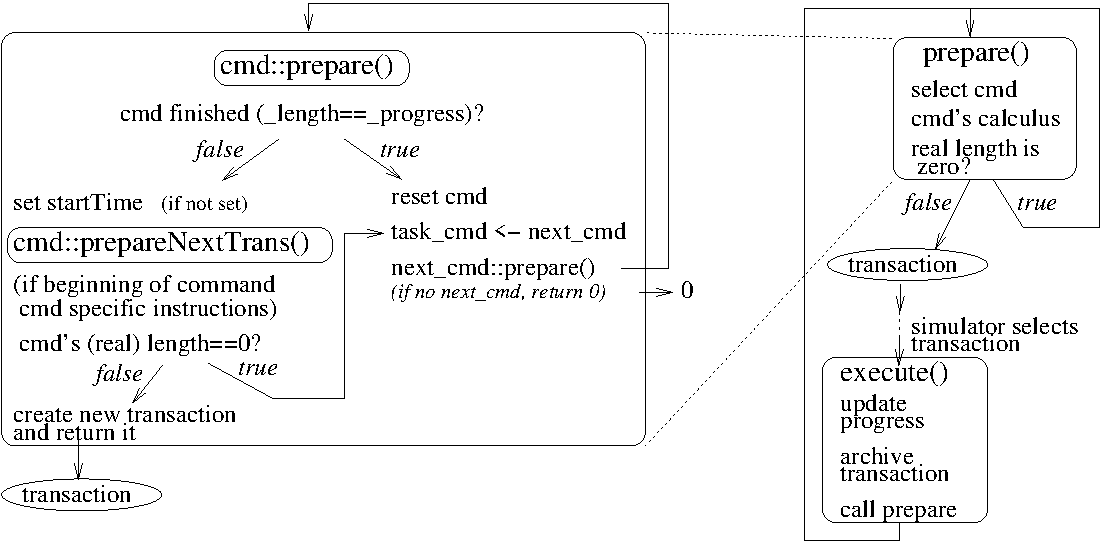
\includegraphics[width=15.5cm]{images/prepare.pdf}

\vspace{1.5mm}\noindent
Calling \cod{prepare} runs consecutive commands until finding one that requires a transaction (non null real length), then build the transaction and sets it as current transaction of the task. It is called on all tasks at the beginning of simulation, and then, when a transaction is executed (selected by the simulator loop), on the transaction's command, to prepare the following transaction w.r.t. control flow.
%===========================================
\class{Task}{WorkloadSource}
note: \cod{schedule} does nothing. Instances also comprise command-specific function (such as length computation for example) which are called by some command' s methods.

%-----------------------
\variable{\_priority} priority of the task
%-----------------------
\variable{\_endLastTransaction} End of the last scheduled transaction of the task
%-----------------------
\variable{\_firstCommand} first command of the task
%-----------------------
\variable{\_currCommand} current command of the task
%-----------------------
\variable{\_isDaemon} flag
%-----------------------
\variable{\_justStarted} true until the first transaction of a task is executed
%-----------------------
\method{addTransaction(iTrans)} Adds transaction to the transaction list of the command. Updates \cod{\_endLastTransaction} with {\tt iTrans}'s end time and unsets \cod{\_justStarted}.
%-----------------------
\method{finished()} Is called when a stop command is encountered. Sets \cod{\_justStarted}.
%-----------------------
\method{getNextTransaction(iEndSchedule)} Returns \cod{\_currCommand}'s current transaction
%-----------------------
\method{getCPU(),getFPGA()}
%£££££££££££££££££££££££££££££££££££££££££££££££££££££££££££££££££££££
\subsection*{Commands}
First, see \cod{TMLCommand} above.
%===========================================
\class{TMLActionCommand}{TMLCommand}
%-----------------------
\variable{\_actionFunc} pointer to the function that implementss command's specific action.
%-----------------------
\method{prepareNextTransaction()} Calls \cod{\_actionFunc}, then makes task change to next command and call \cod{prepare(false)}.
%-----------------------
\method{execute()} does nothing

%===========================================
\class{TMLChoiceCommand}{TMLCommand}
%-----------------------
\variable{\_rangeFunc} pointer to the condition function returning the index of the next command.
%-----------------------
\method{prepareNextTransaction()} makes task change to next command and then call \cod{pre\-pa\-re(false)}.
%-----------------------
\method{execute()} does nothing
%-----------------------
\method{getNextCommands()} selects next command by calling \cod{\_rangeFunc}.

%===========================================
\class{TMLRandomChoiceCommand}{TMLChoiceCommand}
%-----------------------
\variable{\_randomValue} in fact in {\tt IndeterminismSource.h}, no true implementtion (??)
%-----------------------
\method{prepareNextTransaction()} change \cod{\_randomValue} by calling \cod{\_rangeFunc}. then similar to \cod{TMLChoiceCommand}
%-----------------------
\method{execute()} does nothing
%-----------------------
\method{getNextCommands()} returns \cod{\_nextCommand[\_randomValue]}

%===========================================
\class{TMLDelayCommand}{TMLCommand}
%-----------------------
\variable{\_actionFunc} pointer to the function that increments \cod{\_endLastTransaction} with delay duration for passive delays.
%-----------------------
\method{getActiveDelay(), isDelayTransaction()} are redefined
%-----------------------
\method{prepareNextTransaction()} when \cod{\_progress} is 0 (beginning of command), calls \cod{\_ac\-tionFunc} and then, if \cod{length} is 0, makes task change to next transaction and returns \cod{prepare(false)} (this should not happend as \cod{prepareNextTransaction()} seems to be always called with \cod{\_length}$\neq$\cod{\_progress}).\\ Then updates \cod{\_currTransaction} with new one of length \cod{\_length}$-$\cod{\_progress}, and start time \cod{\_endLastTransaction}.
%-----------------------
\method{execute()} increments \cod{\_progress} with \cod{\_currTransaction}'s virtual length, then add \cod{\_curr\-Transaction} to task and calls \cod{prepare(false)}.

%===========================================
\class{TMLExeciCommand}{TMLCommand}
%-----------------------
\variable{\_lengthFunc} pointer to a function computing the length of the command.
%-----------------------
\method{prepareNextTransaction()} Similar to \cod{TMLDelayCommand} except that when \cod{\_prog\-ress} is 0 (beginning of command), updates \cod{\_length} using \cod{\_lengthFunc} instead of calling \cod{\_actionFunc}.
%-----------------------
\method{execute()} Similar to \cod{TMLDelayCommand}

%===========================================
\class{TMLExeciRangeCommand}{TMLCommand}
Similar to \cod{TMLExeciCommand} except that \cod{\_lengthFunc} has range parameters.

%===========================================
\class{TMLNotifiedCommand}{TMLCommand}
determines the number of events queued in a channel. length: fixed constant.
%-----------------------
\variable{\_channel} Channel on which the event is conveyed
%-----------------------
\variable{\_resultVar} number of sample in the channel updated by \cod{execute}.
%-----------------------
\method{prepareNextTransaction()} Updates \cod{\_currTransaction} with new one, with length \cod{\_length}$-$\cod{\_progress}, start time \cod{\_endLastTransaction} and \cod{\_channel}.
%-----------------------
\method{execute()} Similar to \cod{TMLDelayCommand}, moreover sets \cod{\_resultVar} to \cod{\_channel}'s content (amount of messages).

%===========================================
\class{TMLRandomCommand}{TMLCommand}
%-----------------------
\variable{\_rangeFunc} Function returning the range allowed by the command in output parameters {\tt oMin} and {\tt oMax}.
%-----------------------
\variable{*\_resultVar} pointer to the variable in which the random number is put by \cod{prepare\-NextTransaction()}.
%-----------------------
\method{prepareNextTransaction()} Updates \cod{\_resultVar} with generated random number and change task current command to next one before calling \cod{prepare(false)} for this new command.
%-----------------------
\method{execute()} does nothing

%===========================================
\class{TMLReadCommand}{TMLCommand}
%-----------------------
\variable{\_lengthFunc} Function returning the length of the command.
%-----------------------
\variable{\_channel} Channel which is read
%-----------------------
\method{prepareNextTransaction()} When \cod{\_prog\-ress} is 0 (beginning of command), updates \cod{\_length} using \cod{\_lengthFunc} and taking \cod{\_channel}'s width into account (and if length is 0,\ldots\ c.f. \cod{TMLExeciCommand}). Then updates \cod{\_currTransaction} with new one, with length \cod{\_length}$-$\cod{\_progress}, start time \cod{\_endLastTransaction} and \cod{\_channel}. Finally calls \cod{\_channel}'s \cod{testread()} method.
%-----------------------
\method{execute()} Similar to \cod{TMLDelayCommand}, moreover calls \cod{\_channel}'s \cod{read()} method.

%===========================================
\class{TMLWaitCommand}{TMLCommand}
%-----------------------
\variable{\_channel} Channel on which the event is conveyed
%-----------------------
\variable{\_paramFunc} function (\cod{f(param)}) that sets variables of command profile to values provided by {\tt param}. 
%-----------------------
\method{prepareNextTransaction()} Updates \cod{\_currTransaction} with new one, with length \cod{\_length}$-$\cod{\_progress}, start time \cod{\_endLastTransaction} and \cod{\_channel}. Then calls \cod{\_chan\-nel}'s \cod{testread(\_currTransaction)} method. Moreover, for request channels,  if progress is 0 then \cod{\_task->finished()} is called which sets task's \cod{\_justStarted}. 
%-----------------------
\method{execute()} Similar to \cod{TMLDelayCommand}, moreover calls \cod{\_channel}'s \cod{read()} method.

%===========================================
\class{TMLWriteCommand}{TMLCommand}
%-----------------------
\variable{\_lengthFunc} Function returning the length of the command.
%-----------------------
\variable{\_channel} Channel which is written
%-----------------------
\method{prepareNextTransaction()} Similar to \cod{TMLReadCommand} except that \cod{testwrite()} is called instead of \cod{testRead()}.
%-----------------------
\method{execute()} Similar to \cod{TMLDelayCommand}, moreover calls \cod{\_channel}'s \cod{write()} method.

%===========================================
\class{TMLSendCommand}{TMLCommand}
%-----------------------
\variable{\_paramFunc} Function returning the the command parameter.
%-----------------------
\variable{\_channel}  (array of) channels conveying the desired signals
%-----------------------
\method{prepareNextTransaction()} Updates \cod{\_currTransaction} with new one, with length \cod{\_length}$-$\cod{\_progress}, start time \cod{\_endLastTransaction} and \cod{\_channel}. Then calls \cod{\_chan\-nel}'s \cod{testwrite(\_currTransaction)} method.
%-----------------------
\method{execute()} similar to \cod{TMLWriteCommand}.

%===========================================
\class{TMLRequestCommand}{TMLCommand}
%-----------------------
\variable{\_paramFunc} Function returning the parameter of the command.
%-----------------------
\variable{\_channel} Channel on which the request is conveyed.
%-----------------------
\method{prepareNextTransaction()} Similar to \cod{TMLSendCommand}
%-----------------------
\method{execute()} Similar to \cod{TMLSendCommand}

%===========================================
\class{TMLSelectCommand}{TMLCommand}
%-----------------------
\variable{\_channel} array of channels conveying the desired signals
%-----------------------
\variable{\_indexNextCommand} Index of the next command within the \cod{\_nextCommand} array
%-----------------------
\variable{\_paramFuncs} array of parameter function pointers (\cod{\_indexNextCommand} used as index)
%-----------------------
\variable{\_maxChannelIndex} Highest index of the channels on which the \cod{testRead()} method has been performed

%-----------------------
\method{getNextCommand()} returns \cod{\_nextCommand[\_indexNextCommand]}
%-----------------------
\method{getChannel(iIndex)}  if \cod{\_currTransaction} is 0 then returns \cod{\_channel[\_indexNext\-Command]} else returns \cod{\_currTransaction}'s channel.
%-----------------------
\method{prepareNextTransaction()} create a new \cod{\_currTransaction} with length: \cod{\_length}$-$ \cod{\_progress} and start time: tasks's \cod{\_endLastTransaction}.\\ Then, makes \cod{testRead(\_currTransaction}) on channels until finding one that can read, and sets \cod{\_maxChannelIndex} to its index. At the end, if not 0, \cod{\_maxChannelIndex} points to a channel with an available event. Note: \cod{testRead} sets transaction's channel.
%-----------------------
\method{execute()} Cancel read transaction on all channels before cod{\_maxChannelIndex} (or, if 0, \cod{\_nbOfNextCmds}. One browsed channel must be readable, otherwise "error"). Update \cod{\_indexNextCommand} with found index. Updates \cod{\_progress}. Then, adds transaction to task, resets \cod{\_maxChannelIndex} and calls \cod{prepare(false)}. {\bf\textit{Warning}:} if event's length is greather than 1, a transaction may begin on a channel and continue on another one.
%===========================================
\class{TMLStopCommand}{TMLCommand}
%-----------------------
\method{prepareNextTransaction()} Calls \cod{\_task->finished()} and returns 0.
%-----------------------
\method{execute()} does nothing

%@@@@@@@@@@@@@@@@@@@@@@@@@@@@@@@@@@@@@@@@@@@@@@@@@@@@@@@@@@@@@@@@@@@@@
\section*{Directory \cod{arch}}
	
%===========================================
\class{WorkloadSource}{}
Base class for components providing workload like tasks and scheduler
%-----------------------
\variable{workloadList} List of sources which provide transactions to the scheduler

%-----------------------
\variable{\_priority} Priority of the workload source

%-----------------------
\method{getNextTransaction} returns the next scheduled transaction.

%-----------------------
\method{schedule(iEndSchedule)} virtual method. return allocated time slice.

%===========================================
\class{RRScheduler}{WorkloadSource}
Round Robin Scheduler (used for buses and CPUs)
%----------------------- 
\variable{\_nextTransaction} Next transaction to be executed

%-----------------------
\variable{\_timeSlice} Time slice which is granted to ressources

%-----------------------
\variable{\_minSliceSize} Minimum size of a time slice

%-----------------------
\variable{\_elapsedTime} Consumed portion of a time slice

%-----------------------
\variable{\_lastSource} Last workload source to which ressource access was granted

%-----------------------
\method{schedule(iEndSchedule)} updates \cod{\_nextTransaction}(virtual length of new \cod{\_next\-Transaction} is not 0) , \cod{\_lastSource} and \cod{\_elapsedTime}.
For this, schedules the sources and selects the one whose \cod{\_nextTransaction} has the lowest runnable time.\\ Exception (only if new  \cod{\_lastSource}'s transaction is not a static delay): last source is kept if scheduler's \cod{\_nextTransaction} was 0 (is it possible?) or equal to  new  \cod{\_lastSource}'s transaction, or if time remains in timeslice for \cod{\_lastSource}.

%===========================================
\class{RRPrioScheduler}{WorkloadSource}
Round Robin Scheduler with priority (used for CPUs)
%----------------------- 
\variable{\_nextTransaction} Next transaction to be executed

%-----------------------
\variable{\_timeSlice} Time slice which is granted to ressources

%-----------------------
\variable{\_minSliceSize} Minimum size of a time slice

%-----------------------
\variable{\_elapsedTime} Consumed portion of a time slice

%-----------------------
\variable{\_lastSource} Last workload source to which ressource access was granted

%-----------------------
\method{schedule(iEndSchedule)} Similar to previous one, except that for transactions that are not in the future, priority applies.

%===========================================
\class{PrioScheduler}{WorkloadSource}
Scheduler with priority (used for buses)
%----------------------- 
\variable{\_nextTransaction} Next transaction to be executed

%-----------------------
\variable{\_lastSource} Last workload source to which ressource access was granted

%-----------------------
\method{schedule(iEndSchedule)} Similar to previous one.

%===========================================
\class{StrictPrioScheduler}{WorkloadSource}
Scheduler with (preemptive) priority (used for CPUs)
%----------------------- 
\variable{\_nextTransaction} Next transaction to be executed

%-----------------------
\variable{\_timeSlice} Time slice which is granted to ressources

%-----------------------
\variable{\_minSliceSize} Minimum size of a time slice

%-----------------------
\variable{\_elapsedTime} Consumed portion of a time slice

%-----------------------
\variable{\_lastSource} Last workload source to which ressource access was granted

%-----------------------
\method{schedule(iEndSchedule)} a more prior task always preempts.

%===========================================
\class{ScedulableDevice}{}

%-----------------------
\variable{\_simulatedTime} static. Class variable holding the simulation time.

%-----------------------
\variable{\_transactList}	List containing all already scheduled transactions.

%-----------------------
\variable{\_nextTransaction} next transaction to be executed

%-----------------------
\method{schedule()} (virtual. ) Determines the next transaction to be executed.\\ (update \cod{\_nextTransaction})

%-----------------------
\method{addTransaction(iTransToBeAdded)} returns bool if done. Adds the transaction determined by the scheduling algorithm to the internal list of scheduled transactions.

%-----------------------
\method{getNextTransaction()} Returns the transaction determined by the scheduling algorithm (\cod{\_nextTransaction})


%-----------------------
\variable{\_endSchedule} End time of the last scheduled transaction (\cod{\_lastTransaction} in CPU)

%-----------------------
\variable{\_scheduler} internal scheduler, generally invocated by \cod{schedule}.

%===========================================
\class{CPU}{SchedulableDevice}

%-----------------------
\variable{\_taskList} List of all tasks running on the CPU

%-----------------------
\variable{\_lastTransaction} last transaction which has been executed

%-----------------------
\variable{\_busMasterList} List of bus masters

%-----------------------
\variable{amountOfCore} Amount of cores

%-----------------------
\method{virtual truncateAndAddNextTransAt(iTime), truncateNextTrans(iTime)} c.f. \cod{SingleCoreCPU}.

%===========================================
\class{SingleCoreCPU}{CPU}

%-----------------------
\variable{\_busMasterList} list of busmaster of the CPU
	
%-----------------------
\method{getMasterForBus(master)} returns the CPU's bus master associated to the bus of master (obtained by getBus, de facto, first bus of master's \cod{\_busArray}).

%-----------------------
\variable{\_lastTransaction} Last executed transaction.

%-----------------------
\variable{\_nextTransaction} Currently selected transaction (not yet executed).

%-----------------------
\method{calcStartTimeLength(iTimeSlice)} in \cod{\_nextTransaction}, update start time, length, penalties (round to full cycles when required) and transType. In CPU, update \cod{\_masterNextTransac\-tion} (to master of first bus of channel, if exists) and register transaction for this master. 
\begin{itemize}
\item update start time as the maximum of CPU's \cod{\_endSchedule} and \cod{\_runnableTime} of \cod{\_nextTransaction}.
\item update length (only if not bus transaction else it is computed elsewhere) as the minimum of \cod{\_nextTransaction}'s virtual length and \cod{iTimeSlice}.
\item updates \cod{\_taskSwitchingPenalty} and \cod{\_idlePenalty} (for this, compare start time and \cod{\_endSchedule}).
\item sets \cod{\_transType} to \cod{NOCOMM\_TRANS}, \cod{CHANNEL\_TRANS} or \cod{BUS\_TRANS\_NoLength} depending on wether \cod{\_nextTransaction} is, respectively, "without communication", "with communication but without bus" or "with communication and bus".
\item updates \cod{\_masterNextTransaction} and registers \cod{\_nextTransaction} for this master if \cod{\_nextTransaction} is communication. 
\end{itemize}

%-----------------------
\method{getNextTransaction} returns \cod{\_nextTransaction} except if some master before \cod{\_mas\-terNextTransaction} is not granted. Otherwise returns 0. Moreover, if all buses of a communication transaction have been granted (\cod{\_mas\-terNextTransaction} is the last master of the channel), then the length of the transaction is updated w.r.t. its (up to date) virtual length.

%-----------------------
\variable{\_masterNextTransaction} Current bus master for \cod{\_nextTransaction} if it is communication transaction, else 0.

%-----------------------
\method{addTransaction} Adds \cod{\_nextTransaction} to the internal list of scheduled transactions (return true), except if \cod{\_nextTransaction} is a not terminated channel transaction (return false: not all busses of the channel have been handled).

If \cod{\_nextTransaction} is communication,
	\begin{itemize}
	  \item If next master exists (return false), update \cod{\_masterNextTransaction} to next master and register the transaction for this new master.
	  \item Otherwise (return true), add \cod{\_nextTransaction} to all relevant masters ans slaves. Update bus contention.
	\end{itemize}
If "return true",
	\begin{itemize}
	  \item update \cod{\_endSchedule} with end time of \cod{\_nextTransaction}\\
	  update \cod{\_simulatedTime} if it is lower than \cod{\_nextTransaction}'s end time (only if we are not at the end of a daemon task)
	  \item execute \cod{\_nextTransaction}'s command, i.e. in short: increment task progress with transaction's virtual length and add transaction to task.
	  \item add transaction to CPU's transaction list.
	  \item Set \cod{\_lastTransaction} to \cod{\_nextTransaction}. Set \cod{\_nextTransaction} to 0.
	\end{itemize}
%-----------------------
\method{schedule(iEndSchedule)} Call scheduler and update \cod{\_nextTransaction}. If transaction has changed,\\
- call \cod{calcStartTimeLength}\\
- call \cod{\_masterNextTransaction->registerTransaction(0)} if relevant (does not change \cod{\_masterNextTransaction} pointer).

%-----------------------
\method{truncateAndAddNextTransAt(iTime)} called when the execution of a transaction by the simulator may have unblocked a communication transaction on this CPU. Schedule the CPU and if \cod{\_next\-Transaction} have changed, then truncate original one at {\tt iTime}, \cod{addTransaction(0)} and \cod{calcStart\-TimeLength} to update new one. This is done only if the current \cod{\_nextTransaction} is not a bus transaction.

%-----------------------
\method{truncateNextTransAt(iTime)} called by \cod{truncateAndAddNextTransAt} to truncate \cod{\_next\-Transaction}. It computes new length of transaction and updates transaction with this length.

%-----------------------
\method{truncateNextTrans(iTime)} Makes the same work as \cod{truncateAndAddNext\-TransAt} and \cod{truncateAndAddNextTransAt} together, but also truncates bus transactions when it is relevant. Yet not used (selection of algorithm depends on a test which is always true at the beginning of \cod{truncateAndAddNextTransAt})

%===========================================
\class{MultiCoreCPU}{ScedulableDevice}

%-----------------------
\variable{\_busMasterList} list of busmaster of the CPU

%-----------------------
\method{getMasterForBus(master)} returns the CPU's bus master associated to the bus of master (obtained by getBus).
%-----------------------
\variable{coreNumber} core having the lowest end schedule date.

%-----------------------
\variable{multicore} {\ttfamily Cores $\rightarrow$ Dates}, associates end schedule dates to core numbers.

%-----------------------
\method{getMinEndSchedule} return the minimal end schedule date of \cod{multicore}.\\ Set \cod{coreNumber} to the corresponding core.

%-----------------------
\variable{channelEndTime}{\ttfamily Channel $\rightarrow$ Dates}, associates

%-----------------------
\variable{\_lastTransaction} Last executed transaction.

%-----------------------
\variable{\_nextTransaction} Currently selected transaction (not yet executed).

%-----------------------
\method{calcStartTimeLength(iTimeSlice)} in \cod{\_nextTransaction}, update start time, length, penalties (round to full cycles when required) and transType. In CPU, update \cod{\_masterNextTransac\-tion} (to master of first bus of channel, if exists) and register transaction for this master. 
\begin{itemize}
	\item update start time as the maximum of CPU's \cod{\_endSchedule},\cod{\_nextTransaction}'s \cod{\_runnableTime} and \cod{\_nextTransaction}'s channel's \cod{channelEndTime}.
	\item update length (only if not bus transaction else it is computed elsewhere) as the minimum of \cod{\_nextTransaction}'s virtual length and \cod{iTimeSlice}.
	\item updates \cod{\_taskSwitchingPenalty} and \cod{\_idlePenalty} (for this, compare start time and \cod{\_endSchedule}).
	\item sets \cod{\_transType} to \cod{NOCOMM\_TRANS}, \cod{CHANNEL\_TRANS} or \cod{BUS\_TRANS\_NoLength} depending on wether \cod{\_nextTransaction} is, respectively, "without communication", "with communication but without bus" or "with communication and bus".
	\item updates \cod{\_masterNextTransaction} and registers \cod{\_nextTransaction} for this master if \cod{\_nextTransaction} is communication. 
\end{itemize}

%-----------------------
\method{getNextTransaction} returns \cod{\_nextTransaction} except if some master before \cod{\_mas\-terNextTransaction} is not granted. Otherwise returns 0.
%-----------------------
\variable{\_masterNextTransaction} Current bus master for \cod{\_nextTransaction} if it is communication transaction, else 0.
%-----------------------
\method{addTransaction} Adds \cod{\_nextTransaction} to the internal list of scheduled transactions (return true), except if \cod{\_nextTransaction} is a not terminated channel transaction (return false: not all busses of the channel have been handled).

If \cod{\_nextTransaction} is communication,
\begin{itemize}
	\item If next master exists (return false), update \cod{\_masterNextTransaction} to next master and register the transaction for this new master.
	\item Otherwise (return true), add \cod{\_nextTransaction} to all relevant masters ans slaves. Update bus contention.
\end{itemize}
If "return true",
\begin{itemize}
	\item Select a core (update \cod{\_nextTransaction} with it), and updates \cod{multicore} for the selected core with end time of \cod{\_nextTransaction} if it is greater than the current end time associated to this core. The selected core is \cod{coreNumber} except if \cod{\_lastTransaction} and \cod{\_nextTransaction} belong to the same task and the end time of \cod{\_lastTransaction} is lower than the start time of \cod{\_nextTransaction}, in which case the selected core  is the one of  \cod{\_lastTransaction}.
	\item update \cod{\_endSchedule} with \cod{getMinEndSchedule}\\
	update \cod{\_simulatedTime} if it is lower than \cod{\_nextTransaction}'s end time (only if we are not at the end of a daemon task)
	\item execute \cod{\_nextTransaction}'s command, i.e. in short: increment task progress with transaction's virtual length and add transaction to task.
	\item add transaction to CPU's transaction list.
	\item Set \cod{\_lastTransaction} to \cod{\_nextTransaction}. Update \cod{channelEndTime} associated to \cod{\_nextTransaction}'s channel with \cod{\_nextTransaction}'s end time (if relevant). Set \cod{\_nextTransaction} to 0.
\end{itemize}
%-----------------------
\method{schedule(iEndSchedule)} Call scheduler and update \cod{\_nextTransaction}. If transaction has changed,\\
- call \cod{calcStartTimeLength}\\
- call \cod{\_masterNextTransaction->registerTransaction(0)} if relevant (does not change \cod{\_masterNextTransaction} pointer).

%-----------------------
\method{truncateAndAddNextTransAt(iTime)} identical to \cod{SingleCoreCPU}.

%-----------------------
\method{truncateNextTransAt(iTime)} identical to \cod{SingleCoreCPU}

%-----------------------
\method{truncateNextTrans(iTime)} identical to \cod{SingleCoreCPU}

%===========================================
\class{SchedulableComDevice}{SchedulableDevice}

%-----------------------
\method{getBurstSize} Returns the size of an atomic bus transaction

%-----------------------
\method{registerTransaction()} Signals the component that a new transaction has become available and thus rescheduling is needed

%-----------------------
\variable{\_channelBasedPrio} Flag indicating whether bus master based or channel based priorities are used to arbitrate the bus

%-----------------------
\method{virtual calcStartTimeLength(iTimeSlice)} Updates start time (may increase but not decrease) and virtual length (may decrease but not increase).
%-----------------------
\method{virtual calcLength()} Updates length w.r.t virtual length, i.e. increase (but not decrease) length if relevant.

%===========================================
\class{Bus}{SchedulableCommDevice}

%-----------------------
\variable{\_scheduler} Workload sources are busmasters (set in {\tt appmodel.cpp}).

%-----------------------
\variable{\_schedulingNeeded} Dirty flag of the current scheduling decision. Set by \cod{addTransac\-tion} and \cod{registerTransaction}. Unset by \cod{schedule}.

%-----------------------
\method{schedule()} Determines the next bus transaction to be executed. For this, call its internal scheduler (\cod{\_scheduler->schedule(\_endSchedule)}), update \cod{\_nextTransaction}, limits its virtual length w.r.t. burst size, and call \cod{calcStartTimeLength} with the obtained time slice. Unset \cod{\_schedulingNeeded}.

%-----------------------
\method{calcStartTimeLength(iTimeSlice)} Updates the start time and the virtual length of \cod{\_nextTransaction}. Start time updated to \cod{\_endschedule} if greather than current start time. Update virtual length taking bus characteristics into account (decreases if the computed virtual length is smaller than the current one). Increments slave and if new slave exist, then call \cod{\_calcStartTimeLength} of slave (which does nothing).

%-----------------------
\method{calcLength(iTimeSlice)} Updates the length of the transaction considering the virtual length and bus caracteristics? The length of \cod{\_nextTransaction} is increased if the computed length is greater than the current one.
%-----------------------
\method{addTransaction(iTransToBeAdded)} return {\tt true}. Adds the parameter transaction (supposed to be similar to the transaction determined by the scheduling algorithm?) to the internal list of scheduled transactions. Set \cod{\_endSchedule} to the end time of \cod{\_nextTransaction} and \cod{\_nextTransaction} to 0. Set the \cod{\_schedulingNeeded} flag.

%-----------------------
\method{registerTransaction()} Add a transaction waiting for execution to the internal list. ({\_schedulingNeeded=true; \_nextTransaction=0;})

%-----------------------
\method{getNextTransaction()}
	return \_nextTransaction after calling scheduling if required (w.r.t. \cod{\_schedulingNeeded})
	
%===========================================
\class{Slave}{}

%-----------------------
\method{CalcTransactionLength(iTrans)} virtual.

%-----------------------
\method{addTransaction(iTrans)} virtual.

%===========================================
\class{BusMaster}{WorkloadSource}

%-----------------------
\variable{nbOfBuses, \_busArray, \_busSortArray} \cod{\_busArray} points to the bus the master is connected to. \cod{} has the same content, sorted w.r.t. schedule end time.

%-----------------------
\variable{\_nextTransaction}

%-----------------------
\variable{\_nextBus} Next bus pointer

%-----------------------
\variable{\_channelBasedPrioEnabled, \_channelBasedPrio} Flag indicating whether channel based priorities apply and Channel based priority if applicable.\\ (\cod{\_channelBasedPrio} initialized to \cod{\_busArray[0]->ChannelBasedPrio()}).

%-----------------------
\method{registerTransaction(iTrans)} if {\tt iTrans} is not already \cod{\_nextTransaction},\\ set \cod{\_nextTransaction} to {\tt iTrans} and register transaction on any bus (of \cod{\_busArray}). If relevant, set \cod{\_channelBasedPrio} to {\tt iTrans}'s channel's Priority.

%-----------------------
\method{getNextTransaction(iEndSchedule)} returns \cod{\_nextTransaction} except if it is the \cod{\_nextTransaction} of one of the busses (then return 0).

%-----------------------
\method{accessGranted()} returns true if \cod{\_nextTransaction}$\neq$0 and is the \cod{\_nextTransaction} of a bus (schedule the busses while checking). Set \cod{\_nextBus} to the one of these bus with the lowest end schedule date. 

%-----------------------
\method{getBus()} \cod{\_busArray[0]}

%-----------------------
\method{getNextBus()} returns current value of \cod{\_nextBus} which is always \cod{\_busArray[0]} in current implementation (but may be changed by \cod{accessGranted} when considering multibuses--not implemented).

%-----------------------
\method{addTransaction(iTransToBeAdded)} Add transaction to \cod{\_nextBus} and set \cod{\_next\-Tran\-saction} to 0.

%@@@@@@@@@@@@@@@@@@@@@@@@@@@@@@@@@@@@@@@@@@@@@@@@@@@@@@@@@@@@@@@@@@@@@
\section*{Directory \cod{sim}}
%===========================================
\class{Simulator}{}

%-----------------------
\method{channelImpactsCommand(iCh,iCmd)} Checks if command may be impacted by a anction on a channel, i.e. if {\tt iCh} belongs to {\tt iCmd}'channels.

%-----------------------
\method{getTransLowestEndTime(oResultDevice)} Returns the transaction with the lowest end time proposed by CPU schedulers. Iters \cod{\_getNextTransaction} on CPU (and FPGA) list and compare lowest end time of these transactions to find result.

%-----------------------
\method{simulate(oLastTrans)} call \cod{prepare} on current command (initial one) of each task. Schedule all CPUs (and FPGAs). Run the following main loop untill stop flag or no more transaction on non-daemon task. Return the last executed transaction. The loop:
\begin{itemize}
	\item get transaction \cod{T} with lowest end time and its associated device \cod{D}.
	\item \cod{T->addTransaction(0)}, which may update \cod{\_masterNextTransaction} (to next master) and return false when \cod{T} is communication. In this case, the loop is terminated.\\
	Otherwise, continue with next items. While doing this, the transaction is "executed" (which prepares its following transaction) and may unblock communication command waiting for data or write space to be available.
	\item for each task \cod{t} on another CPU (or FPGA) \cod{C} whose current (communication) command may be unblocked by (communication) \cod{T}, if \cod{t} is not the current task of its associated CPU (or FPGA) then
	\begin{itemize}
	\item if \cod{C} has no current transaction, then it is scheduled.
	\item Otherwise \cod{C->truncateAndAddNextTransAt(T->getEndTime())} is called. This schedule \cod{C} and if \cod{C}'s \cod{\_nextTransaction} changes, the original one is truncated at \cod{T}'s end time and added, i.e. it is terminated at the current date. Currently, bus transactions are not truncated but the algorithm that does this is implemented (\cod{CPU::truncateNextTrans}) and could be made operational by small modifying at the beginning of \cod{CPU::truncateAndAddNextTransAt}.
	\end{itemize}
	\item schedule \cod{D}
\end{itemize}

\section*{Remarks about communication transactions on channels}
\begin{itemize}
	\item As length of a data communication transaction is known late (approximately when the transaction is ready to execute), it may be selected by the simulator loop earlier than it should be (simulated transactions are not always ordered w.r.t. their endTime).
	\item \cod{Bus}'schedulers are called by \cod{Bus}'s \cod{getNextTransaction} which is called by \cod{BusMas\-ter}'s \cod{getNextTransaction} and \cod{BusMaster}'s \cod{accessGranted}.\\
	\cod{Bus}'schedulers call \cod{calcStartTimeLength} which updates the virtual length of the transaction but not the length.
	\item \cod{getNextTransaction} returns \cod{\_nextTRansaction} only if it is not the \cod{\_next\-Trans\-ac\-tion} of one of the busses. Not sure that this method is called anywhere (searched and not found\ldots).
	\item \cod{accessGranted} is called by CPU's \cod{getNextTransaction} and access is granted if \cod{\_nextTRansaction} is also the \cod{\_nextTransaction} of one of the busses of the master.
	\item Story of a channel-bus transaction:
	  \begin{enumerate}
	  	\item \cod{\textit{Communication}Command}'s \cod{prepareNextTransaction} create the transaction.\\ The transaction is provided  with a runnable time and an initial virtual length which takes channel state into account. All task's initial commands are "prepared" at initialisation, and then, each time a transaction (having an associated command) is executed by the simulator loop, to produce the (control flow relative) following transaction.
	  	\item transaction is chosen for the first time by the \cod{CPU}'s scheduler in which a call to
	  	\cod{CPU}'s \cod{calcStartTimeLength} sets \cod{\_masterNextTransaction} to first master and registers the transaction for this master. At this point, transaction's timings are not set (keep their initial value, 0). And all channel's bus  until \cod{\_masterNextTrans\-action} are (trivially) granted (as there are none).
	  	\item  Transaction (and \cod{CPU}) is selected by simulator, after verifying that all bus masters until \cod{\_masterNextTransaction} (included) have been granted. Indeed \cod{getLowest\-Transac\-tionEndTime} calls \cod{getNextTransaction} on each CPU and this \cod{getNext\-Trans\-action} only select a data communication transaction if bus masters before \cod{\_masterNext\-Trans\-action} are granted. Verifying that buses are granted invokes their scheduling (if required) which updates the virutal length of the transaction w.r.t. bus constraints. If \cod{\_masterNextTransaction} is the last master of the channel, the virtual length is up to date and thus, the length of the transaction can be computed: it is updated to its final value.(*)
	  	\item \cod{addTransaction} is called and
	  	\begin{enumerate}
	  		\item either \cod{\_masterNextTrransaction} is the last master of the channel and the transaction is executed: the transaction is added to all masters and slaves of the channel. This is the end of the story.
	  		\item or \cod{\_masterNextTrransaction} is not the last master of the channel. Then \cod{\_masterNextTrransaction} is set to the following one and the transaction is registered for this new master. 
	  	\end{enumerate}
	  	\item If the story is not terminated (point (b) above) then, return to 3 (possibly after some simulator loop iterations on other CPUs), the transaction is selected again and then point 4 above is executed again. executing point 3 again schedules the new \cod{\_masterNextTrransaction} which may update start time and virtual length (and length if last master) of the transaction.
	  \end{enumerate}

\end{itemize}
(*) Notice that the length is only known at this moment, thus before this moment the transaction may be selected by \cod{getLowest\-Transac\-tionEndTime}, although its endTime is not the lowest one (it is not a problem(?)).
\section*{Figures}
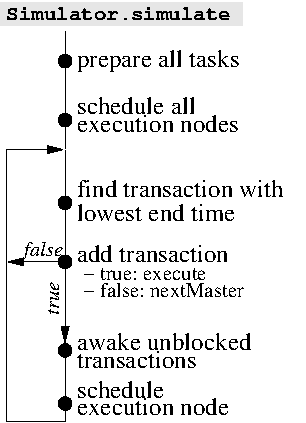
\includegraphics[width=6cm]{images/simulate.pdf}\hspace{5mm}
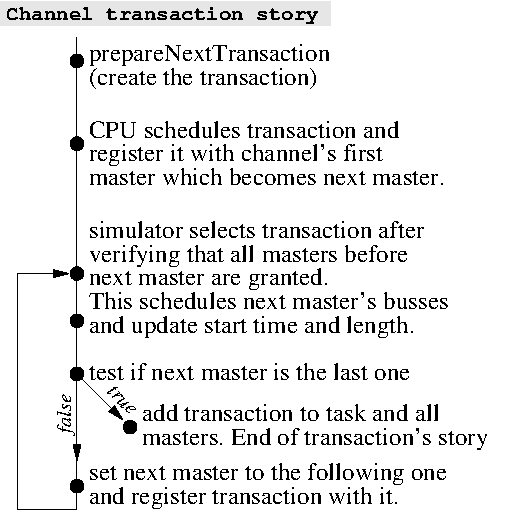
\includegraphics[width=9cm]{images/channelTrans.pdf}

\vspace{5mm}
\includegraphics[width=15.5cm]{images/ClassDiag1.pdf}

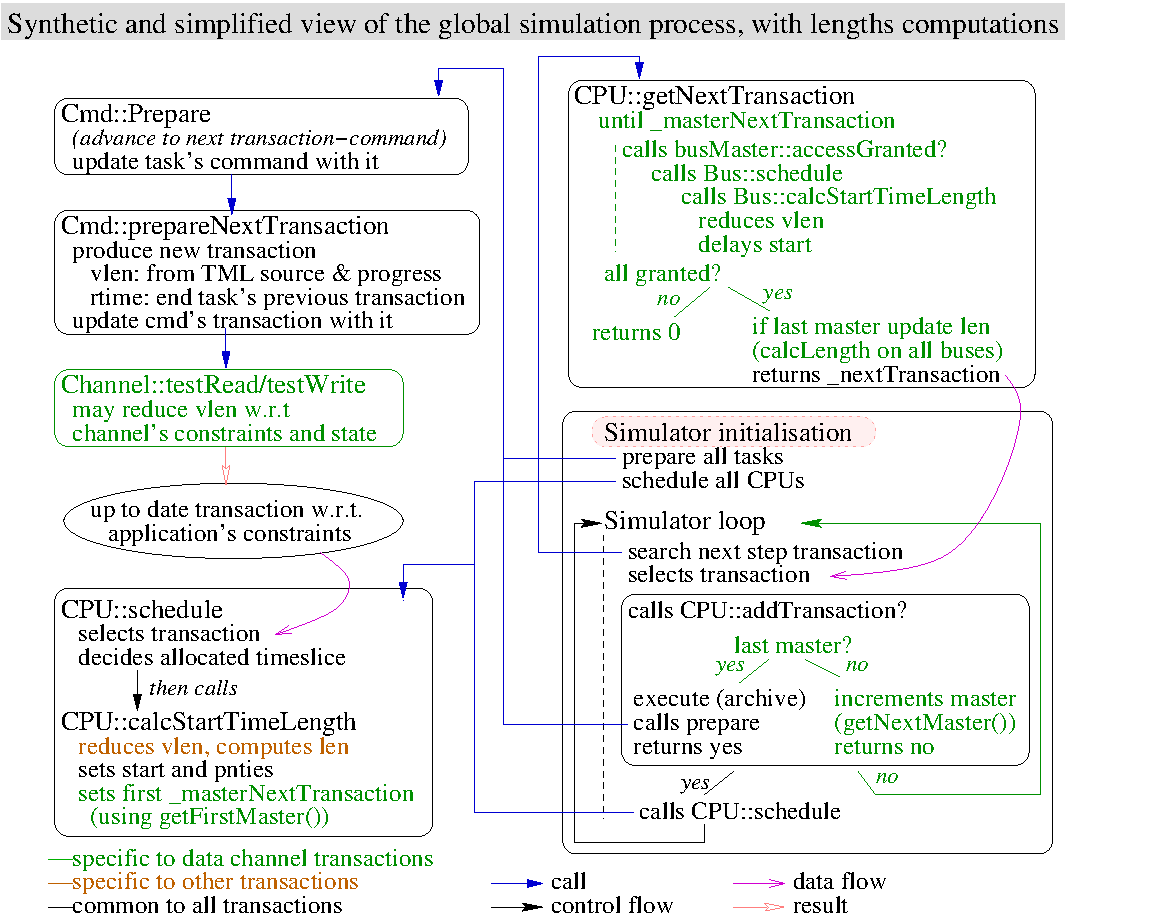
\includegraphics[width=15.5cm]{images/busTime.pdf}


\end{document}

